\documentclass[12pt]{article}

\usepackage{graphicx}
\usepackage{paralist}
\usepackage{hyperref}
\usepackage{xspace}
\usepackage{amsfonts}
\usepackage{amsmath}

\newcommand{\latex}{\LaTeX\xspace}

\oddsidemargin 0mm
\evensidemargin 0mm
\textwidth 160mm
\textheight 200mm
\renewcommand\baselinestretch{1.0}

\pagestyle {plain}
\pagenumbering{arabic}

\newcounter{stepnum}

\title{Requirements Specification}
\author{COMP SCI 2XB3, Lab 02, Group 05}

\begin {document}

\maketitle

\section {The Domain}

This project aims to track historic crime data of major cities and generate commuting routes that will avoid high crime areas while reducing trip durations. Areas avoided will consists of crimes that are frequent, violent, and severe. The goal for our implementation is to provide users with a more informed perspective of travel methods so that they can take necessary precautions as they see fit. We will implement our project first as a web application, later transitioning into a mobile version once fundamental operations are optimised. \\

In the early stages of our application we aim to focus strictly on the Greater Toronto Area. Once an efficient model has been developed for this geographic region we plan to expand to other major cities across North America.\\

	Stakeholders for our application consist mainly of individuals in the regions covered by our application. Those who choose to use our product will have a fuller understanding of their environment giving them the opportunity to keep themselves and others out of harm’s way. Those who don’t use our product might notice a change in volume of traffic in given areas of their commute.\\
	
	Our product may give users information that encourages them to change their commuting patterns. Entities that may be affected by this change consist of local transit services and businesses. If a given area sees a significant increase or decrease in traffic, local transit services might need to consider modifying the resources they offer to reflect new commuter preferences. This shift in commuting preferences might also have an affect on store traffic for businesses established near an area that has been deemed a crime hotspot.

\section {Functional Requirements}
Step safe will take an input of a starting location and destination, and output directions between the two locations. Formulation of this output will be done by considering the fastest route first, and then making additional adjustments to avoid areas of high crime. 

%UML
\section* {UML Diagram}

\begin{center}
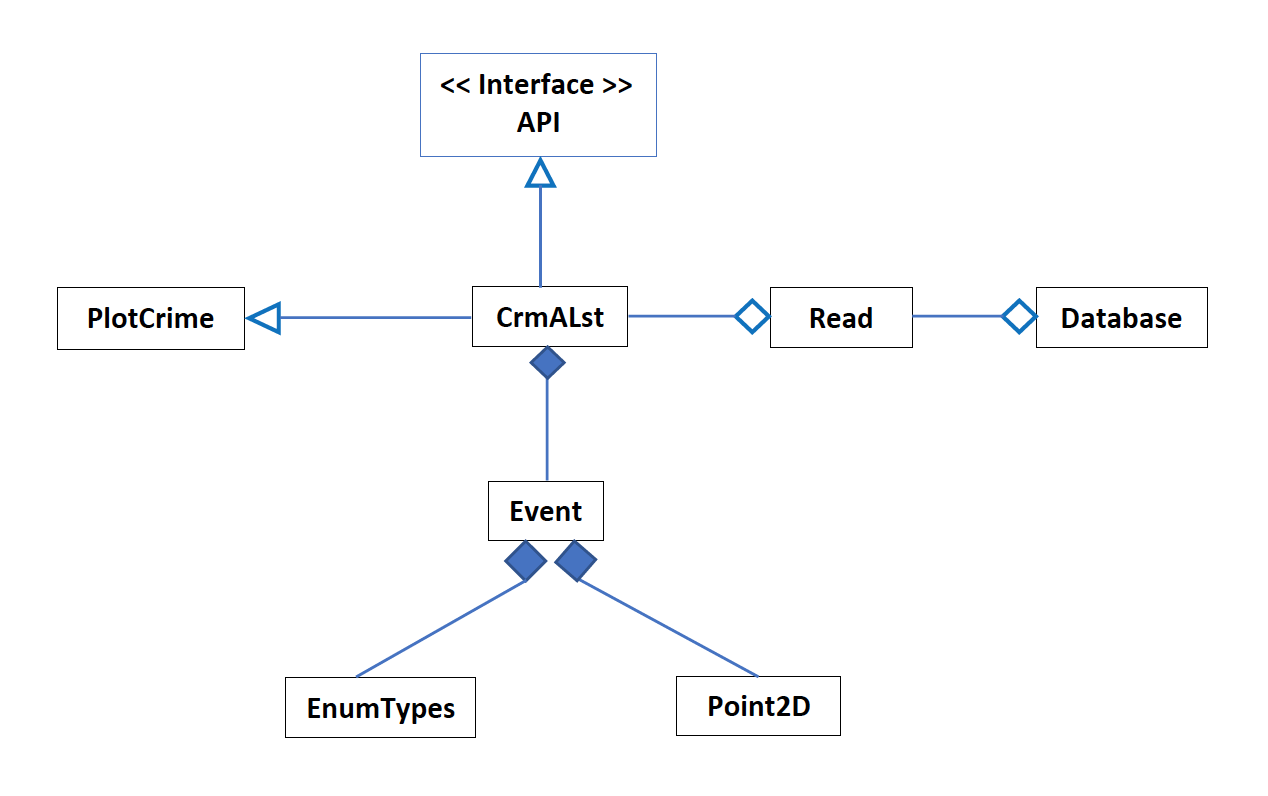
\includegraphics[scale = 0.65]{UML.png}
\end{center}
 
\newpage



\section* {Fundamental Types Module}

\subsection*{Module}

FundamentalTypes

\subsection* {Description}
This module consists of fundamental supporting data types for crime information.

\subsection* {Uses}

TimeADT(s, h)

\subsection* {Syntax}

\subsubsection* {Exported Constants}

None

\subsubsection* {Exported Types}

CoordinateT = tuple of (x : float , y : float)     where x is \text{Latitude}, y is \text{Longitude}\\
MCI = \{assault, breakAndEnter, robbery\}\\ 
Premise = \{outside, house, commercial, apartment, other\}\\
Hood =  tuple of  (id : $\mathbb{N}$, area : String)\\
~\\
CrimeInfoT = tuple of (time: TimeADT(s, h), place: Premise, \\
coordinate: CoordinateT, type: MCI, neighbourhood: Hood)

\subsubsection* {Exported Access Programs}

None

\subsection* {Semantics}

\subsubsection* {State Variables}

None

\subsubsection* {State Invariant}

None

\subsubsection* {Assumptions}

None

\newpage

\section* {Occurrence Time ADT Module}

\subsection*{Template Module}

TimeADT(s, h)

\subsection*{Description}
The module provides the abstract data type for the occurrence time of crimes.

\subsection* {Uses}

None

\subsection* {Syntax}

\subsubsection* {Exported Constants}

None

\subsubsection* {Exported Types}

TimeADT = ?

\subsubsection* {Exported Access Programs}

\begin{tabular}{| l | l | l | p{5cm} |}
\hline
\textbf{Routine name} & \textbf{In} & \textbf{Out} & \textbf{Exceptions}\\
\hline
new SeqADT & s : string, h : string  & TimeADT & InvalidArguments\\
\hline
getYear & ~ & int & ~\\
\hline
getMonth & ~ & int & ~\\
\hline
getDay & ~ & int & ~\\
\hline
getHour& ~ & int & ~\\
\hline
toWeekDay & ~ & WeekDays & ~\\
\hline
compareTo & TimeADT & int & ~\\
\hline
toString & ~ & string & ~\\
\hline
\end{tabular}

\subsection* {Semantics}

\subsubsection* {State Variables}

$year$: integer\\
$month$: integer\\
$day$: integer\\
$hour$: integer\\

\subsubsection* {State Invariant}

$month \in [1..12]$ \\
$hour \in [0..24]$ \\
output of $compareTo \in [-1, 0, 1]$ 

\subsubsection* {Assumptions}

The input string $s$ should be the format: $yyyy-mm-dd$ where year, month and day are separated by dash.\\

\subsubsection* {Access Routine Semantics}

\noindent new TimeADT($s, h$):
\begin{itemize}
\item transition: $year :=$ extract year information from input s and convert to integer
\\$~~~~~~~~~~~~~~~~month :=$ extract month information from input s and convert to integer
\\$~~~~~~~~~~~~~~~day :=$ extract day information from input s and convert to integer
\\$~~~~~~~~~~~~~~~hour := (integer) h$
\item output: $out := \mbox{self}$
\item exception: $(\text{day not in the range of the month}  \Rightarrow \text{InvalidArgument})$
\end{itemize}

\noindent getYear():
\begin{itemize}
\item output: $out := year$
\item exception: none
\end{itemize}

\noindent getMonth():
\begin{itemize}
\item output: $out := month$
\item exception: none
\end{itemize}

\noindent getDay():
\begin{itemize}
\item output: $out := day$
\item exception: none
\end{itemize}

\noindent getHour():
\begin{itemize}
\item output: $out := hour$
\item exception: none
\end{itemize}


\noindent toWeekDay():
\begin{itemize}
\item output: $out := \text{day of a week}$
\item exception: none
\end{itemize}


\noindent compareTo:
\begin{itemize}
\item output: $i, out := $ -1, 0, 1 respectively if t1 is before, equal, after t2
\item exception: none
\end{itemize}

\noindent toString():
\begin{itemize}
\item output: $out := $ string representation of the time in the format: $yyyy-mm-dd:hh$
\item exception: None
\end{itemize}

\subsubsection* {Local Types}
WeekDays = \{Monday, Tuesday, Wednesday, Thursday, Friday, Saturday, Sunday\}\\


\newpage

\section* {Crime Data Association List Module}

\subsection*{Module}

CrmALst

\subsection*{Description}
The module provides an abstract object to store crime records.

\subsection*{Functionalities}
$add$ - add a crime record to the sequence\\
$remove$ - remove a crime record from the sequence\\
$elm$ - check if a crime record exists in the sequence\\
$info$ - returns the detailed information of a crime\\
$count$ - count the number of crimes which satisfy the property given by the input function

\subsection* {Uses} 

FundamentalTypes\\
TimeADT(s, h)\\
GetCrmRate

\subsection* {Syntax}

\subsubsection* {Exported Constants}

None

\subsubsection* {Exported Types}

FundamentalTypes

\subsubsection* {Exported Access Programs}

\begin{tabular}{| l | l | l | p{5cm} |}
\hline
\textbf{Routine name} & \textbf{In} & \textbf{Out} & \textbf{Exceptions}\\
\hline
init & ~ & ~ & ~\\
\hline
add & string, CrimeInfoT & ~ & KeyError\\
\hline
remove & string & ~ & KeyError\\
\hline
elm & string & $\mathbb{B}$ & ~\\
\hline
info & string & CrimeInfoT & KeyError\\
\hline
count & $\text{CrimeInfoT} \rightarrow \mathbb{B}$ & integer &\\
\hline
sort & ~ & \text{sequence of string} &\\
\hline

\end{tabular}

\subsection* {Semantics}

\subsubsection* {State Variables}

$s$: sequence of CrimeT

\subsubsection* {State Invariant}

None

\subsubsection* {Assumptions}

CrmALst.init() is called before any other access program.

\subsubsection* {Access Routine Semantics}

\noindent init():
\begin{itemize}
\item transition: $s := \{ \}$
\item exception: none
\end{itemize}

\noindent add($id$, $i$):
\begin{itemize}
\item transition: $s := s \cup \{ \langle id, i \rangle \}$
\item exception: $(\langle id, ? \rangle \in s \Rightarrow \text{KeyError} )$
\end{itemize}

\noindent remove($id$):
\begin{itemize}
\item transition: $s := s - \{ \langle id, i \rangle \}$ where $\langle id, i
  \rangle \in s$
\item exception: $(\langle id, i \rangle \notin s \Rightarrow \text{KeyError} )$
\end{itemize}

\noindent elm($id$):
\begin{itemize}
\item output: $out := \langle id, i \rangle \in s$
\item exception: none
\end{itemize}

\noindent info($id$):
\begin{itemize}
\item output: $out := i$ where $\langle id, i \rangle \in s$
\item exception: $(\langle id, i \rangle \notin s \Rightarrow \text{KeyError} )$
\end{itemize}

\noindent count($f$):
\begin{itemize}
\item output: $out := (+ i: \text{CrimeInfoT} | i \in CrimeInfoT \wedge f(i) : 1)$
\item exception: None
 \end{itemize}
 
 \noindent sort:
\begin{itemize}
\item output: $out := $ a sequence of crime IDs which is sorted by ascending order based on the crime of the around area gotten by applying $getCrime$ function on its CrimeInfoT
\item exception: None

\end{itemize}


\subsection*{Local Types}

CrimeT = tuple of (id: string, info: CrimeInfoT)

\newpage

% to do: Sort
\section* {Get Crime Module}

\subsection*{Module}

GetCrm

\section* {Description}
The module provides the function to calculate the number of crimes in the around area of a coordinate.

\subsection* {Uses}

FundamentalTypes\\
TimeADT(s, h)\\
CrmALst

\subsection* {Syntax}

\subsubsection* {Exported Constants}

None

\subsubsection* {Exported Types}

None

\subsubsection* {Exported Access Programs}
\begin{tabular}{| l | l | l | l |}
\hline
\textbf{Routine name} & \textbf{In} & \textbf{Out} & \textbf{Exceptions}\\
getCrime & $id: \mbox{string}, r: \mathbb{R} $& integer & ~\\
\hline
getCoordinate & $id: \mbox{string} $& CoordinateT & ~\\
\hline
\end{tabular}

\subsection* {Semantics}

\subsubsection* {Environment Variables}
s : sequence of CrimeT, generated by CrmALst


\subsubsection* {State Variables}
None

\subsubsection* {State Invariant}
None

\subsubsection* {Assumptions}

The argument $r$ is the radius of the circle which represents the range of the around area. It's specified by unit $kilogram$.

\subsubsection* {Access Routine Semantics}

\noindent getCoordinate($id$):
\begin{itemize}
\item output: $out := i.coordinate$ where $\langle id', i \rangle \in s \wedge id' = id$
\item exception: none
\end{itemize}

\noindent getCrime(id, r):
\begin{itemize}
\item transition: $s := (+ (id', i): \text{CrimeT} | \text{getCoordinate}(id') \in circle(c, r): 1)$ where $c$ = getCoordinate(id)
\item exception: none
\end{itemize}

The function $getCrime$ do searching on $s$ and count the number of crimes happened in the around area.

\subsection*{Local Functions}
\noindent circle: $\text{CoordinateT} \times \mathbb{R} \rightarrow \text{set of CoordinateT}$\\
\noindent circle ($c$, $r$) $\equiv \{(x, y) : CoordinateT | (x - x_0)^2 + (y - y_0)^2 \le r^2\ : (x, y)\} $ where $c = (x_0, y_0)$



\newpage

\section* {Read Module}

\subsection* {Module}

Read

\subsection* {Description}
The module provides functions to read data from dataset.

\subsection* {Uses}

CrmALst

\subsection* {Syntax}

\subsubsection* {Exported Constants}

None

\subsubsection* {Exported Access Programs}

\begin{tabular}{| l | l | l | l |}
\hline
\textbf{Routine name} & \textbf{In} & \textbf{Out} & \textbf{Exceptions}\\
load\_crime\_data & $s: \mbox{string}$ & ~ & ~\\
\hline
\end{tabular}

\subsection* {Semantics}

\subsubsection* {Environment Variables}

crime\_dataset: csv file containing all crime data

\subsubsection* {State Variables}

None

\subsubsection* {State Invariant}

None

\subsubsection* {Assumptions}

The input file will match the given specification.

\subsubsection* {Access Routine Semantics}

\noindent load\_crime\_data($s$)
\begin{itemize}
\item transition: read data from the file crime\_dataset associated with the string s.
  Use this data to update the state of the CrmALst module.  Load will first
  initialize CrmLst (CrmLst.init()) before filling CrmALst with crime records that
  follows the types in CrimeT.

  The input csv file contains the following fileds:\\
  $x$: lantitude ,  $y$: longitude ,  $event\_unique\_id$: id of the crime , $occurrencedata$: crime occurrence date , 
  $premisetype$: premise type , $offence$: the short stand for MIS (e.g. B\&E for BreakAndRnter), 
  $MIS$: MIS , $Hood\_ID$: hood id , $Neighbourhood$: the area name\\
  
 
\item exception: none
\end{itemize}


\newpage
%to do: Graph
\section* {Graph Module}

\subsection*{Module}

Graph

\subsection*{Description}
Graph a sequence of coordinates on the map.

\subsection* {Uses}

 FundamentalTypes

\subsection* {Syntax}

\subsubsection* {Exported Constants}

None

\subsubsection* {Exported Types}

None

\subsubsection* {Exported Access Programs}

\begin{tabular}{| l | l | l | p{5cm} |}
\hline
\textbf{Routine name} & \textbf{In} & \textbf{Out} & \textbf{Exceptions}\\
\hline
graphSeq & xs : sequence of CoordinateT & ~ & ~\\
\hline
\end{tabular}

\subsection* {Semantics}

\subsubsection* {State Variables}

None

\subsubsection* {State Invariant}

None

\subsubsection* {Assumptions}

None

\subsubsection* {Access Routine Semantics}

\noindent graphSeq(xs):
\begin{itemize}
\item transition: display path connected by $xs$ on the map
\item exception: none
\end{itemize}

\newpage
%to do: API
\section* {API Module}

\subsection*{Module}

API

\subsection*{Description}
The module provide application programming interface for the project.

\subsection* {Uses}

 FundamentalTypes\\
 CrmALst\\
 GetCrm\\
 Graph

\subsection* {Syntax}

\subsubsection* {Exported Constants}

None

\subsubsection* {Exported Types}

None

\subsubsection* {Exported Access Programs}

\begin{tabular}{| l | l | l | p{5cm} |}
\hline
\textbf{Routine name} & \textbf{In} & \textbf{Out} & \textbf{Exceptions}\\
\hline
navigate & $start$ : string, $end$ : string & ~ & WrongLocation\\
\hline
\end{tabular}

\subsection* {Semantics}

\subsubsection* {State Variables}

None

\subsubsection* {State Invariant}

None

\subsubsection* {Assumptions}

None

\subsubsection* {Access Routine Semantics}



\noindent negivate(start, end):
\begin{itemize}
\item transition: display the best route between starting point and destination.
\item exception: none
\end{itemize}

\subsubsection* {Local Functions}
\noindent convertToCoordinade: $\text{string} \rightarrow \text{CoordinateT}$\\
\noindent convertToCoordinade($l$): returns the coordinate of the location given by string $l$

\section {Non-Functional Requirements}
The software should have a dynamic and reasonable trade-off between efficiency and crime avoidance to encourage reliability. The product will originally be available to users in the Greater Toronto Area and accessed through a web application. Individual user information and location will remain hidden from other users to promote security. To increase accuracy of results, the directions outputted will use a function to optimize the crime score and the time to reach the inputted destination. This analysis as well as the sorting and searching algorithms would need to be as efficient as possible to provide a good user experience. Techniques for decreasing speed should be considered to minimize total run time of direction processing. The user interface should be simple and consist of two inputs for the starting and final destinations and one output of the directions. Multiple choices of directions may be presented with different variables considered (such as total distance, toll roads, etc). Outputted directions would provide the users with distances and road names with directions for each turn. 

\section {Requirements on Development and Maintenance Process}

The three main algorithms that StepSafe uses includes a search algorithm, a sort algorithm and a graphing algorithm. Of the three algorithms, the search algorithm has the highest priority because the data generated will be used in the graphing algorithm. The sort algorithm is needed to filter out relevant data to be used. \\

Quality control procedures will include several steps of testing: unit testing, integration testing, system testing, and acceptance testing. All testing, developing, and designing of code will seek to ensure that modules, and ultimately the web application are verifiable, correct, reliable, usable, efficient, and as robust as possible. A unique module will be created for the purpose of facilitating testing. The functions in the module will have meaningful names relating to what is being tested. After running all test cases in the module, there will be a summary of the tests that were run, including number of passed and failed tests. During the development stage, unit testing, both from a blackbox and whitebox perspective will be performed after modification/creation of a function or property of the module, to ensure that the individual units of code work as intended. Integration test will be regularly used, when possible to ensure that new and updated code does not cause any problems. Following the completion of preliminary modules, System testing can be done to ensure the compatibility of our code as a web application. Lastly, acceptance checking will be done prior to web application launch to ensure all requirements are met, and that the application is suitable to be used by the public. This will include testing of the application’s reliability and usability by having our programmers use directions given by the app to traverse areas in the target city. Further testing will also be done by non-programmers outside of the project to gain objective feedback about the web application,that will be considered for update and change. \\

After initial establishment of the web applications, possible future improvements of the application could include different filtering for methods of transportation, and additional features such as time estimation from destination to arrival, options for path optimization for a sequence of destinations, and exporting direction instructions to a mobile phone.\\

In order to ensure that our application is up-to-date with current technology, features and methods will be modularized properly with information hiding so that the application can be easily modified. By doing this, identifying and fixing bugs in code will also be more efficient. Other anticipated changes include possible porting to new hardware or software platforms such as a mobile application version, that can perform the same functionality with more convenience. \\


\end {document}
